\documentclass{mcmthesis}

%------------begin preamble---------------
\usepackage{newtxtext}%\usepackage{palatino}
\usepackage{indentfirst} % first line indent
\def\figureautorefname{Fig.}

%-----------toc specification------------------
\usepackage[nottoc]{tocbibind} % add ref to toc
\setcounter{tocdepth}{2}
\usepackage{setspace}

%-----------float specification------------------
\usepackage{float}
\usepackage[
    font=small, %
    labelfont=bf, %
    textfont=normalfont, %
    labelformat=simple, %
    labelsep=period %
]{caption}
\usepackage[
    font=small, %
    labelfont=normalfont, %
    textfont=normalfont, %
    labelformat=parens, %
    labelsep=space %
]{subcaption}

%------------algo envronment-----------------------
\usepackage{algorithm}
\usepackage{algpseudocode}
\renewcommand{\algorithmicrequire}{\textbf{Input:}}  % Use Input in the format of Algorithm
\renewcommand{\algorithmicensure}{\textbf{Output:}} % Use Output in the format of Algorithm
\makeatletter
\newenvironment{breakablealgorithm}
  {% \begin{breakablealgorithm}
   \begin{center}
     \refstepcounter{algorithm}% New algorithm
     \hrule height.8pt depth0pt \kern2pt% \@fs@pre for \@fs@ruled
     \renewcommand{\caption}[2][\relax]{% Make a new \caption
       {\raggedright\textbf{\ALG@name~\thealgorithm} ##2\par}%
       \ifx\relax##1\relax % #1 is \relax
         \addcontentsline{loa}{algorithm}{\protect\numberline{\thealgorithm}##2}%
       \else % #1 is not \relax
         \addcontentsline{loa}{algorithm}{\protect\numberline{\thealgorithm}##1}%
       \fi
       \kern2pt\hrule\kern2pt
     }
  }{% \end{breakablealgorithm}
     \kern2pt\hrule\relax% \@fs@post for \@fs@ruled
   \end{center}
  }
\makeatother

%-----------lstlisting settings--------------------
\lstset{breaklines =true}
\lstloadlanguages{Python}

%-----------User-defined Macros--------------------
\def\TeamNumber{2112243}
\def\Problem{C}
\def\AGH{Asian Giant Hornet}
\def\VM{Vespa mandarinia}
\def\vm{Vespa mandarinia}
\newcommand{\red}[1]{\textcolor{red}{#1}}

%-----------MCM Template options-------------------
\mcmsetup{
    CTeX = true, % 写中文文档时,设置为 true
    tcn = \TeamNumber,
    problem = \Problem,
    sheet = true,
    titleinsheet = true,
    abstract = true,
    keywordsinsheet = true,
    titlepage = false % 去掉重复的summary page
}

\title{Denoising the Buzz: A Report Analysis Model for Vespa mandarinia Reinforced by Multimodal Data}
%------------end preamble---------------

\begin{document}

%------------begin summary sheet---------------
\begin{abstract}

Since the first discovery of \VM \ in September 2019, Washington State has witnessed several confirmed sightings along with a multitude of mistaken reports from the public, which has exerted a huge burden on government agencies of Washington State. Therefore, it is high time an effective solution should be developed to process the data from public detection reports and reduce the consumption of resources for additional investigation.

To tackle the challenge mentioned above, we propose a multimodal modeling method with full utilization of the data given, including temporal-spatial features as well as the textual and visual data from public reports. Its output scores demonstrate the likelihood of mistaken reports or credible ones, which can help researchers better deal with the tough task.

\textbf{First}, 1. As for temporal-spatial features, we combine the use of grey system model, cellular automaton, and temporal-spatial clustering, to analyze and predict the spread properties and trajectories of \VM; 2. In terms of textual data, the LDA Topic model and naive Bayes algorithm are applied to notes and lab comments, to extract the words of strong correlation with high confidence, detailed description or mistaken possibility; 3. As to visual data, We build a CNN network for image classification and train it on images re-annotated by labels extracted from lab comments. The network can infer the confidence score of submitted photos or videos.

\textbf{Then}, we integrate our multimodal model after normalizing and summarizing the output scores of each component. Evaluation is conducted on the original data set, which eventually implies the strong correlation between the results of out model and the report priorities, and thus the accuracy and helpfulness of the model proposed is proved.

\textbf{Next}, we discuss the situation for updating the model by introducing the concept of model entropy, to represent the influencing factors of the unverified recently-inputted data. The conclusion is that data updates and network retraining are required once the entropy is above the designated threshold, 

\textbf{Finally}, we decide the active threshold of \VM \ sighting reports based on the former analysis. and any report below is considered negative. With the living properties and data analysis taken into consideration, once no more recent report exceeds the threshold over the designated period, it can be regarded that \VM \ has been eradicated in Washington state.


\begin{keywords}
Multimodal modeling; Temporal-Spatial Clustering; the LDA Topic Model; Naive Bayes Method; Image Classification
\end{keywords}
\end{abstract}

\maketitle
%------------end summary sheet---------------

%------------begin table of contents---------------
\begin{spacing}{0.2}
    \tableofcontents
\end{spacing}
\newpage
%------------end table of contents---------------


%============begin thesis (main part)===============
\section{Introduction}
\subsection{Background}

\VM, also known as Asian giant hornet, is an invasive species of hornet as well as a recently invaded alien species to Washington state. They are harmful to local beneficial insects, \emph{e.g.} European honeybees, breaking local ecosystem and thus is regarded as agricultural pests.

Due to its potentially severe impact on the local ecological environment, the government agencies have adopted a series of measures as the responses to the challenge. However, problems have been aroused that the massive amount of reports mistaking another type of insects for \VM \ consumed lots of resources for investigation. Therefore, it's essential for government agencies to adopt measures to address the challenge. 

\subsection{Problem Restatement}

The primary questions for this problem are \textbf{how to interpret the data from public reports} and \textbf{how to prioritize public reports for additional investigation}. More specifically, we need to solve the following problems:

\begin{itemize}
    \item \textbf{Problem 1}: Disscuss the spread of \VM \ over time, and the precision of prediction.
    \item \textbf{Problem 2}: Propose and analyze a multimodal model combining temporal-spatial, textual and visual features from public reports, to predict the likelihood of a mistaken classification.
    \item \textbf{Problem 3}: Prioritize reports with higher likelihood to be positive sightings for additional investigation based on the model proposed.
    \item \textbf{Problem 4}: Discuss the conditions and methods for updating the model proposed, especially from the perspective of time and frequency.
    \item \textbf{Problem 5}: Discuss the conditions for confirming the eradication of \VM in Washington State.
\end{itemize}

\subsection{Our Work}

Our work follows the following workflow framework, as shown in the \autoref{fig:workflow}. The multimodal modeling method utilizes the raw data from different perspectives, including temporal-spatial clustering as well as textual and visual modeling. It then aggregates the features and scores from all three aspects and outputs the final confidence score indicating the likelihood of mistaken reports or credible ones. We call our model START for its four essential parts.

\begin{figure}[h]
    \small
    \centering
    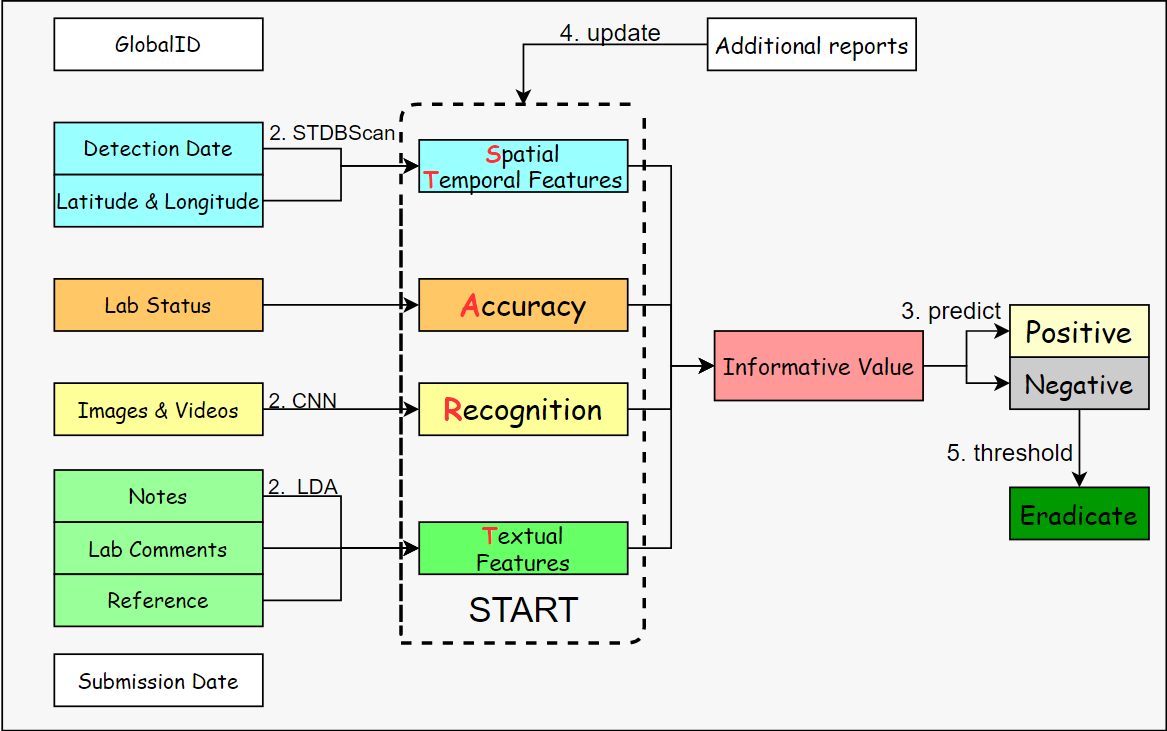
\includegraphics[width=\textwidth]{workflow.png}
    \caption{Workflow framework.} \label{fig:workflow}
\end{figure}

\newpage

\begin{itemize}
    \item In problem 1, we first conduct a preliminary analysis to portrait the overall characteristics of the raw data set. Then based on positive reports, we discuss how to predict the spread of \VM\ in both number growth and geographical distribution points, using grey system model and cellular automaton respectively.
    \item In problem 2, we propose a multimodal model composed of three parts to predict the likelihood of mistaken reports based on the quantitative scores from each part.
        \begin{enumerate}
            \item From the perspective of temporal-spatial data, ST-DBScan, a temporal-spatial clustering algorithm is applied to model the data of detection date and sighting location, which helps us to analyze the spread trajectories of \VM, and then score the other reports according to their deviation with the estimated spread trajectory.
            \item In terms of textual data, We apply the LDA Topic model and naive Bayes algorithm to notes and lab comments, to extract the words of strong correlation with high confidence, detailed description or mistaken possibility, and thus scoring the report notes according to their confidence and helpfulness. \\
            Besides, we also extract the ground truth label of negative reports for the following image classification tasks, since the number of each class in the original data set is of severe imbalance.
            \item As for visual data, with the help of lab comments, we re-split the images into 10 categories including \VM \ and other species of high possibility to be mistaken for. We then build a CNN network and train it on the re-annotated images, which can infer the confidence score of submitted photos or videos.
        \end{enumerate}
    \item In problem 3, we integrate our multimodal model and apply it to the original data set. We normalize and then sum up the scores so that reports with higher scores are more likely to be positive ones. Visualization of results turns out that all positive labeled reports are of high ranks and proves the accuracy and reliability of our model.
    \item In problem 4, we discuss this issue by the situation of lab status. We introduce the concept of model entropy to represent the influencing factors of the unverified new data. If the entropy is above the threshold, data updates and network retraining are required.
    \item In problem 5, based on the ranking result from problem 3, we regard the score of the last positive report with a margin as the active threshold, and any report below is considered negative. If there is no recent report that exceeds the threshold over the period, we considered \VM \ eradicated in Washington state. The life cycle of \VM\ is also taken into consideration.
\end{itemize}


\section{Problem 1: Prediction and Precision}
In this section, we preprocess the data set and analyze the spread of \VM\ over time.
\subsection{Data Cleaning}
We first remove those records whose detection time is earlier than 2019 because the \VM\ was discovered in September 2019. The submission date is mainly decided by the faculty in WSDA and useless for our subsequent analysis so we just simply delete this column. In the end, 
we eliminate 72 unqualified items and leave 14, 2055, 2286 and 2055 items for positive ID, negative ID, unverified and unprocessed data, respectively.

\subsection{Overall Data Characteristics}
We have plotted the number of public reports per month in \autoref{fig:dataset-time-dist} and find that it
peak around September and October, which matches the life cycle of \VM \cite{matsuura1973bionomic} and also
shows that they do exist in the wild. And since \VM\ hibernates in
winter, positive report number drops in November and December, then decreasing to and remaining zero in the
first few months of a year. In terms of the number of negative public reports, its highest value, unlike
that of positive reports, appears in August, as \autoref{fig:dataset-time-dist} has shown. Therefore, the
number of other insects is generally higher in August, that is, there is a certain difference between the life cycle of these native other insects and \VM.

\begin{figure}[ht]
    \centering
    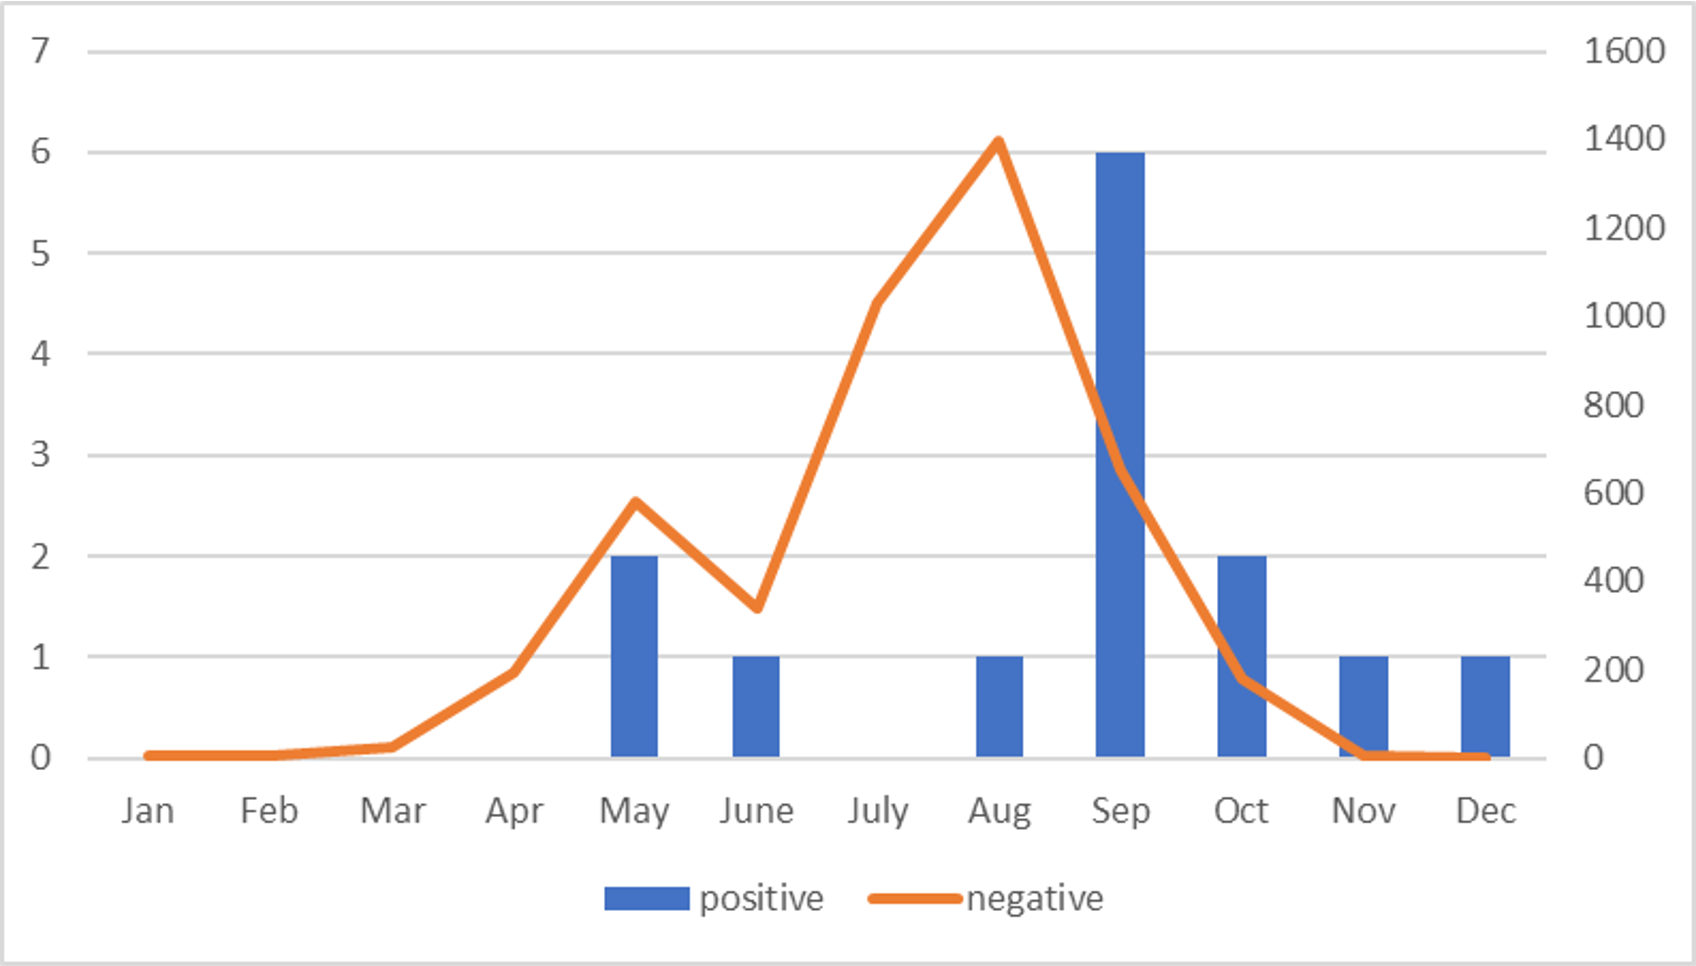
\includegraphics[width=14cm]{dataset-time-dist-new.png}
    \caption{Time distribution (per month) of positive and negative public reports, positive reports
    in blue and corresponding to the left axis, negative ones in orange and corresponding to the right
    axis.}
    \label{fig:dataset-time-dist}
\end{figure}

%\newpage
From a geographical point of view shown in \autoref{fig:dataset-heatmap}, \VM s do not spread far. By
examining longitude and latitude, positives reports form several obvious clusters and distances within each 
cluster are no greater than $\pm 0.5^\circ$ in longitude(around 31 miles) and $\pm 0.2^\circ$ in
latitude(around 12 miles).

\begin{figure}[ht]
    \centering
    \begin{subfigure}{6.8cm}
        \centering
        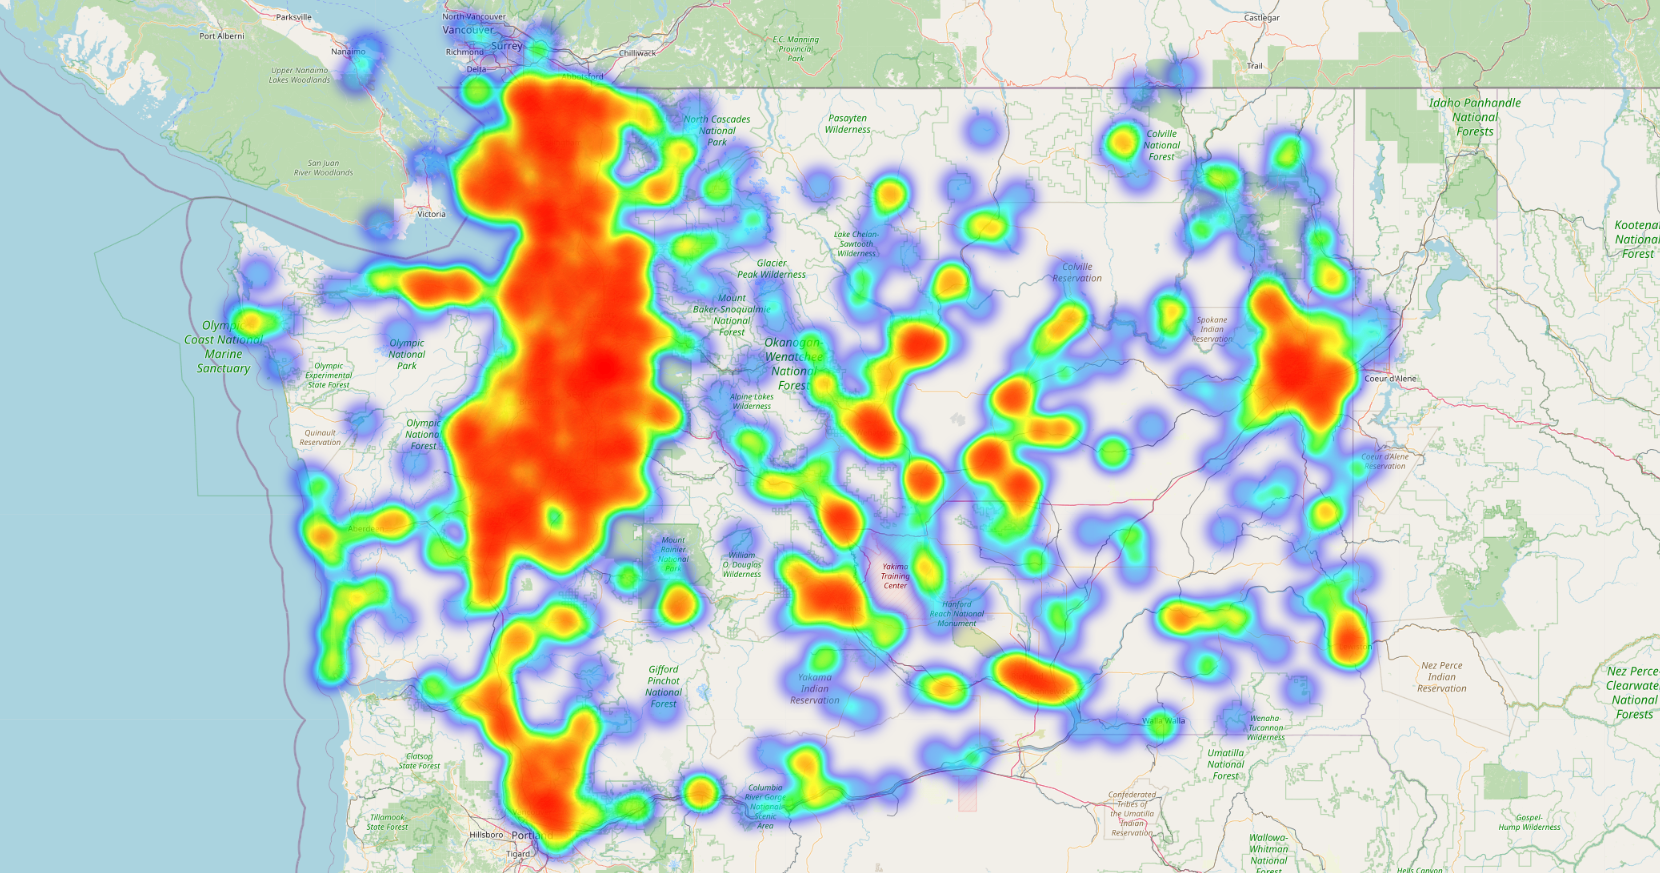
\includegraphics[width=6.8cm]{figures/dataset-heatmap-geo.png}
        \caption{}
        \label{fig:dataset-heatmap-geo}
    \end{subfigure}
    \quad
    \begin{subfigure}{7.37cm}
        \centering
        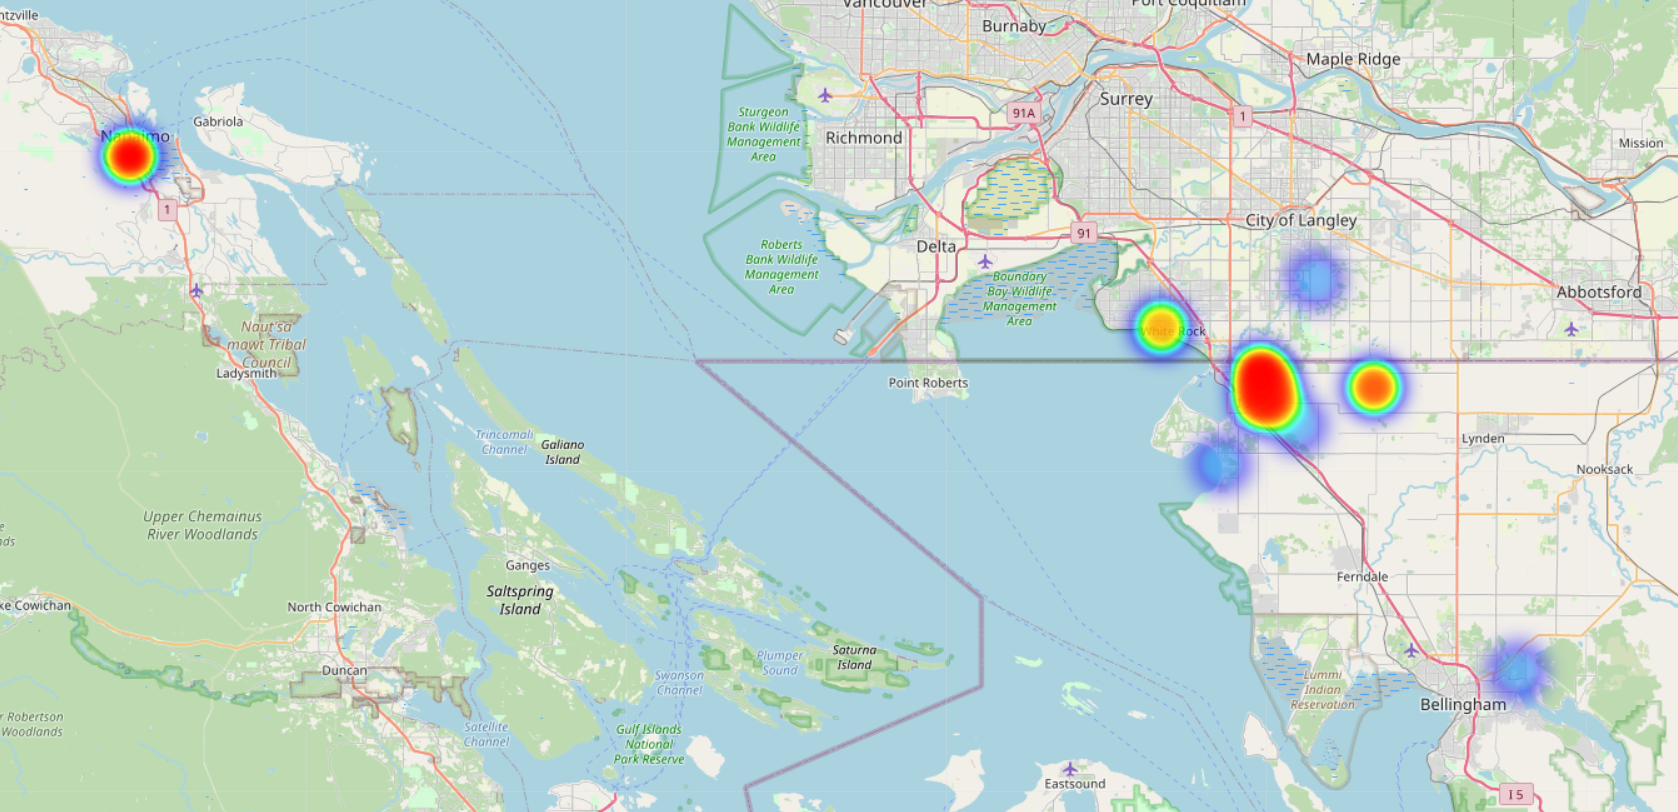
\includegraphics[width=7.37cm]{dataset-heatmap-time}
        \caption{}
        \label{fig:dataset-heatmap-time}
    \end{subfigure}
    \caption{(\subref{fig:dataset-heatmap-geo}) Geographical distribution of all public reports, warmer color meaning higher report density and (\subref{fig:dataset-heatmap-time}) geographical distribution of positive public reports, warmer color meaning report appears later in the year.}
    \label{fig:dataset-heatmap}
\end{figure}

\subsection{Prediction and Precision}
According to the insights we have gained from the sections above, we believe that the spread of \VM\ can be
predicted in the following two aspects:
\begin{itemize}
    \item \textbf{Number growth}: How the number of this pest in a given area would change over time.
    \item \textbf{Geographical distribution}: Which regions are potentially invadable and most likely to succumb.
\end{itemize}

\subsubsection{Prediction on number growth}
Although we have already picked out every positive report from the data set, only 14 \VM\ occurrences can be used to develop our prediction model. Furthermore, occurrence number per month, shown as the blue lines in \autoref{fig:predict-time-dist}, appears to be in a relatively complex pattern that we find it hard to achieve a good performance with traditional algorithms like regression. Therefore, we adopted grey series forecasting methods from the grey system theory to better deal with problems with small amount of data and complicated internal laws\cite{liu2011intro}. More specifically, we have applied both GM(1,1) and GM(2,1) grey differential model on these 14 \VM\ occurrences and trained the two models to predict occurrence number every month. The results are shown as orange lines in \autoref{fig:predict-time-dist}.

\begin{figure}[htbp]
    \centering
    \begin{subfigure}{0.4\textwidth}
        \centering
        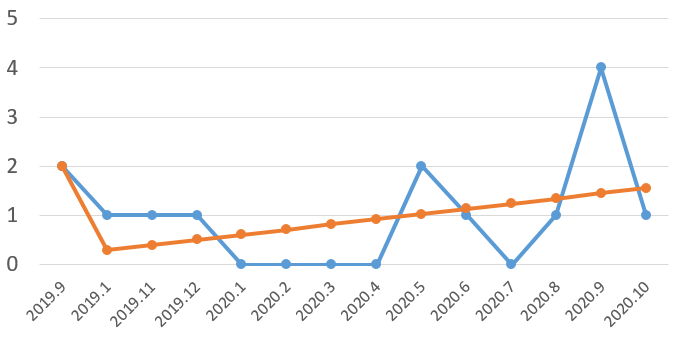
\includegraphics[width=\textwidth]{GM11-predict-time-dist.png}
        \caption{GM(1,1) model prediction results.}
        \label{fig:GM11-predict-time-dist}
    \end{subfigure}
    \quad
    \begin{subfigure}{0.44\textwidth}
        \centering
        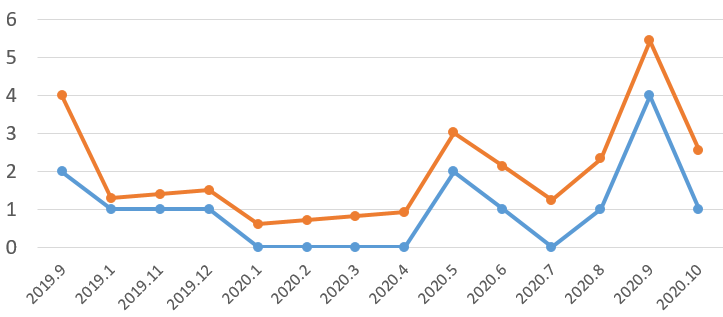
\includegraphics[width=\textwidth]{GM21-predict-time-dist.png}
        \caption{GM(2,1) model prediction results.}
    \label{fig:GM21-predict-time-dist}
    \end{subfigure}
    \caption{Comparing GM(1,1) and GM(2,1) model predictions on the number of \VM\ occurrences per month, blue lines are from the original data set and orange lines are model predictions.}
    \label{fig:predict-time-dist}
\end{figure}

In \autoref{fig:GM11-predict-time-dist}, our forecast results deviate greatly from the real data. That is because the actual occurrence series constantly floats up and down, while GM(1,1) as a first order model is suitable for sequences with strong exponential law and can only describe monotonous changes\cite{julong1989intro}. On the other hand, the second order model GM(2,1) yields predictions with much more acceptable errors, but it is more complicated and harder to implement.


\subsubsection{Prediction on geographical distribution}
Results in \autoref{fig:dataset-heatmap-time} showed that all \VM\ occurrences indicated by positive reports lay very close to each other, not even one degree away in longitude and latitude. For those within the same cluster, calculated straight distances between \VM\ occurrences are no greater than 34 miles. At further examination, it turns out that the 14 occurrences are centralized not only spatially but also temporally: they all occurred within only one year, where it's \VM's annually biological life cycle\cite{matsuura1973bionomic} that dominates their activities and would introduce errors. To address this problem, we searched for some related work and the following is what we have found:

In 2020, Alaniz \emph{et al}. \cite{alaniz2021giants} predicted that in the western coast of the USA,
an environmentally suitable zone, among many others, for \VM\ should appear in the states of Washington, Oregon, and in northern California. They applied ecological niche modeling together with a maximum entropy
algorithm, combining 25 environmental metrics and spatial occurrences of the target species to estimate
the native habitat suitability. After that, native habitat suitability is projected to the USA to find regions with similar environmental characteristics, which are then marked as potential invadable areas. Ecological niche modeling predictions on the spread of invasive species after their recent arrival usually produce a good level of accuracy\cite{peterson2012species,elith2010art}, and the results do match figure \autoref{fig:dataset-heatmap-geo} quite well. Nuñez-Penichet \emph{et al}. \cite{nunez2021geo} obtained similar results through ecological niche modeling as well, but they further conducted several dispersal simulations using cellular automaton algorithm to verify those results and obtained good consistency.

Therefore, we believe that although \VM's short-term geographical distribution is hard to predict, it can still be predicted with an acceptable accuracy in the long term.


\section{Problem 2: Multimodal Data Processing}
\subsection{Spatial Temporal Features}
ST-DBScan\cite{STDBScan} is a efficient density-based clustering algorithm, which has the ability of discovering clusters according to spatial and temporal values of the objects.
\subsubsection{Setup of spatial temporal features}

We apply the ST-DBScan model to positive, negative,  unverified, and unprocessed reports, respectively. The temporal spatial data is constructed as <time, longitude, latitude>, and is fed into the model. The model needs three additional factors.

\begin{enumerate}
\item Eps1: The spatial density threshold (maximum spatial distance) between two points to be considered related. 
\item Eps2: The temporal threshold (maximum temporal distance) between two points to be considered related.
\item Min samples: The number of samples required for a core point.
\end{enumerate}

According to the reference\cite{AGH} document, we conclude that \VM\ queens have a range estimated at 30km for establishing her new nest. Thus, we assign 30km to the largest radius of the activity of \VM. Besides, bees are social animals so the spotting cases within one month are most likely to be the same group of \VM. Finally, we set Eps1, Eps2, and Min samples to 0.3(after unit conversion),30 and 5, respectively.
\begin{figure}[h]
    \centering
    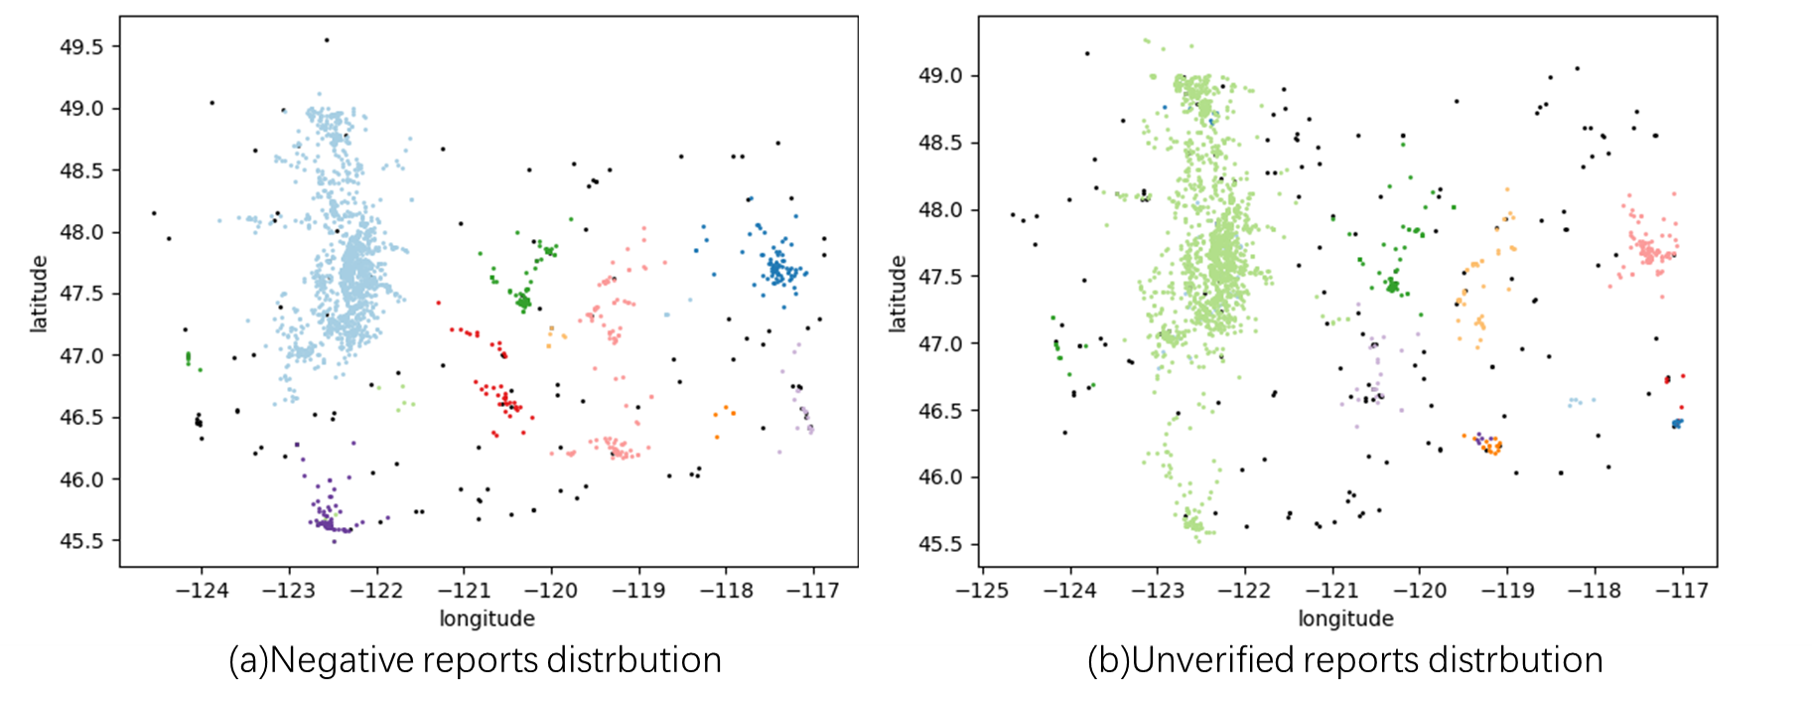
\includegraphics[width=\textwidth]{ST_Neg_unver_30.png}
    \caption{Comparison of the distribution of negative category and unverified category.}
    \label{fig:ST_Neg_unver_30}
\end{figure}

We unexpectedly found that the distribution of negative and unverified data is very similar in \autoref{fig:ST_Neg_unver_30}, and a large amount of data are concentrated in plain areas with relatively low altitudes. It indicates that many records are false sightings.
\subsubsection{Analysis on spatial temporal features}
\label{section:ST_analysis}
The components in ST-DBScan code can be used to value the connections between each other on the maps.

\begin{itemize}
    \item positive/negative category
    $$
    W =
    \begin{bmatrix}
      A_1&A_2  &A_3  &A_4  &A_5&A_6&A_7&A_8 \\
      B_1&B_2  &B_3  &B_4  &B_5&B_6&B_7&B_8 \\
      C_1&C_2  &C_3  &C_4  &C_5&C_6&C_7&C_8 
    \end{bmatrix}
    $$

    We assume that there are eight points, three of which form a cluster and the other five points do not form any cluster. This matrix $W^{3\times8}$ represents the distance between these three core clustering points and all other data. For example, $A_4$ represents the distance between the fourth point and the first point of the three points that have formed a cluster. The smaller the distance, the closer the relationship between the fourth point and the cluster. The distance from the core clustering point itself is 0. We only need to add up all the columns in the matrix and divide by eight to get the aggregation degree of the eight points. Finally, the reciprocal of the value is defined as $ST_{score}$.
    For example, the influential factor of the i-th point is calculated as:
    \begin{equation}
    Score_{ST_i} = 
    \left\{
        \begin{array}{lr}
            \cfrac{1}{\frac{A_i+B_i+C_i+...}{N}} ,\ i\in S_{positive}\\
            -\cfrac{1}{\frac{A_i+B_i+C_i+...}{N}} ,\ i\in S_{negative}
        \end{array}
    \right.
    \end{equation}
    % \begin{eqnarray}
    
    % \frac{1}{\frac{A_i+B_i+C_i+...}{N}} ,\ i\in S_{positive\  or\  negative}
    % \end{eqnarray}
    where N is the total number of points.
    \item unverified/unprocessed category
    
    The next step is to determine the influence of positive and negative reports on neighboring areas. We begin with the idea of gravity. In physics, every particle attracts every other particle in the universe with a force that is directly proportional to the product of their masses and inversely proportional to the square of the distance between their centers:
    \begin{eqnarray}
    F_g\propto \frac{m_1m_2}{r^2} 
    \end{eqnarray}
    Therefore, we define the influence of positive and negative categories on the temporal spatial data of unverified and unprocessed categories as the following formula:
    \begin{eqnarray}
    Score_{ST_i}=\sum_{j\in positive}\gamma^{t_{i,j}}
    \frac{Score_{ST_j}}{r_{i,j}^2}+\sum_{k\in negative}\gamma^{t_{i,k}} \frac{Score_{ST_k}}{r_{i,k}^2},\ i\in S_{unverified\  or\  unprocessed}
    \end{eqnarray}
    where $\gamma$ is a discounted factor of time, and we set it to be 0.999. $r_{i,j}$ is the geographical distance between the i-th point and the j-th point. $t_{i,j}$ is time intervals(Unit: day) between the two reports. Since $Score_{ST}$ of negative report is negative, the latter one is also a negative number.
    
\end{itemize}

\subsection{Textual Features}

We utilize text data from three perspectives, extracting the words of strong correlation with three types including high confidence, detailed description, or mistaken possibility, which are denoted as $CF$, $DT$, $MP$ respectively. The scores are calculated in the manner of the naive Bayes method, which represents the confidence and helpfulness report notes.

Besides, we match the ground truth labels of wasp species likely to be mistaken from lab comments, for the sake of the following image classification task.

\subsubsection{Data processing}

We first merge the data with images and mark each report by whether it is with an image, which implies that the lab comments may not only rely on the report notes. We then generally select features including report notes, lab status, lab comments, and the mark of whether it is with images for text mining. To further utilize the information conveyed by text data, we conduct the following processing methods to texts:

\begin{enumerate}
\item Texts are split into words, and misspellings are corrected.
\item Verbs are lemmatized to a first-person single form, nouns are lemmatized to a single form, and comparative degree and superlative degree of adjectives and adverbs are converted to their basic form.
\item Stopwords and punctuation are removed from sentences.
\item TF-IDF\cite{tfidf} (term frequency–-inverse document frequency) is calculated and the LDA\cite{lda} (Latent Dirichlet Allocation) topic model is applied to the pre-processed data for text mining.
\end{enumerate}

\subsubsection{Insights of text data}

After calculating the TF-IDF score of all the words in the pre-processed report notes, we find out the most frequently used words in report notes, and a wordcloud is generated as shown in \autoref{fig:wordbee-colored}.

\begin{figure}[h]
    \centering
    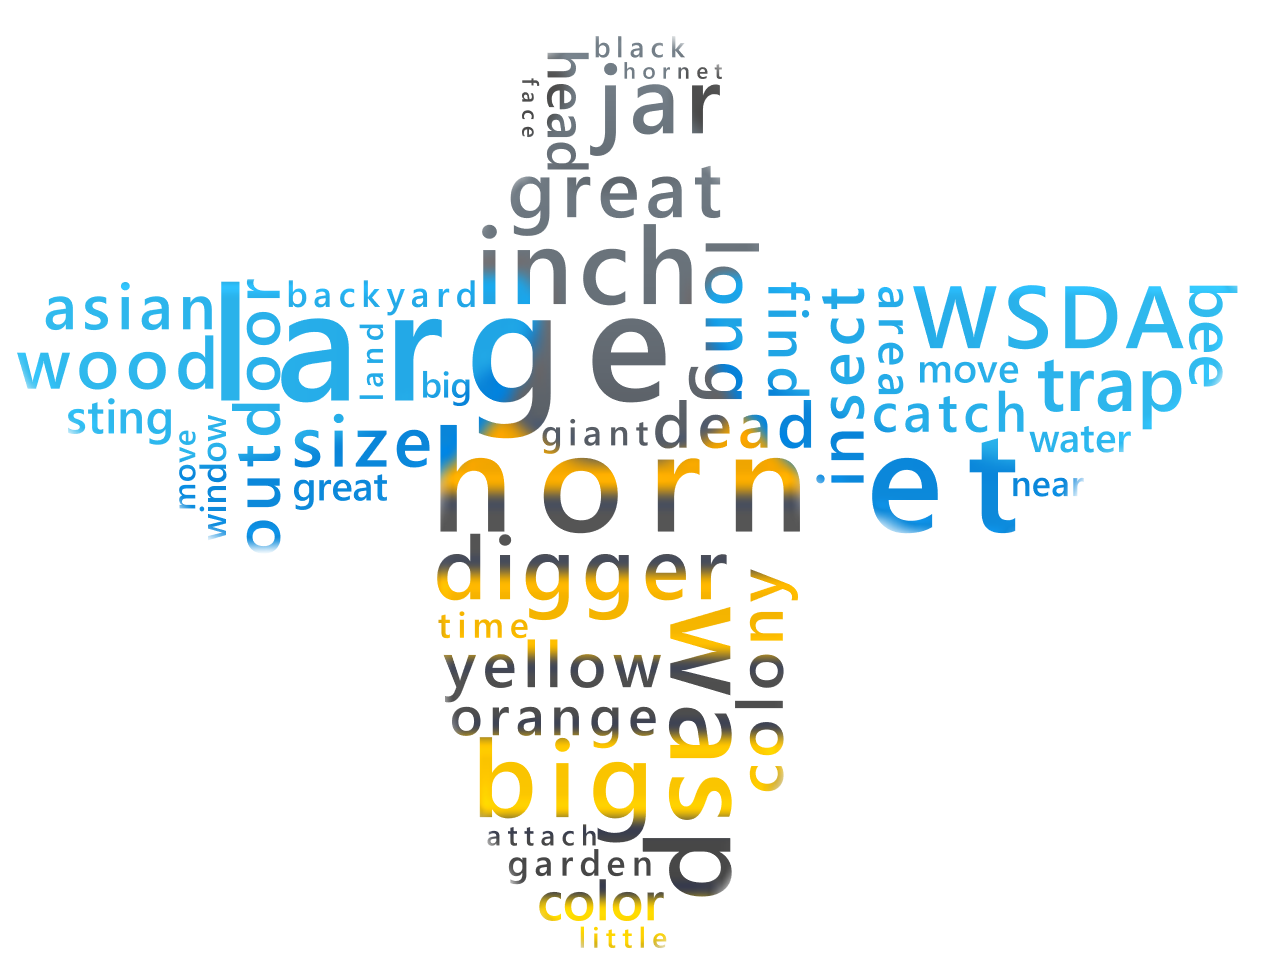
\includegraphics[width=8cm]{wordbee-colored.png}
    \caption{Word cloud generated from report notes.}
    \label{fig:wordbee-colored}
\end{figure}

The TF-IDF score for token $t$ in document $d$ from document set $D$ is calculated as follows:
\begin{eqnarray}
TF\text{-}IDF(t,d,D) = TF(t,d) \times IDF(t,D)
\end{eqnarray}
Where:
\begin{eqnarray}
TF(t,d) = log(1+freq(t,d))
\end{eqnarray}
\begin{eqnarray}
IDF(t,D) = log(\frac{N}{count(d \in D : t \in d)})
\end{eqnarray}

Firstly, we filter out the most frequent words only in positive report notes, which turn out to be words of high professionalism and confidence, \emph{e.g.} "WSDA" may imply that the detection was reported by professional staff of WSDA and thus more reliable, while "specimen" suggests that scientific research has been conducted for the detection. Detailed results Detailed results are shown in \autoref{fig:tfs} (a).

\begin{figure}[htbp]
    \centering
    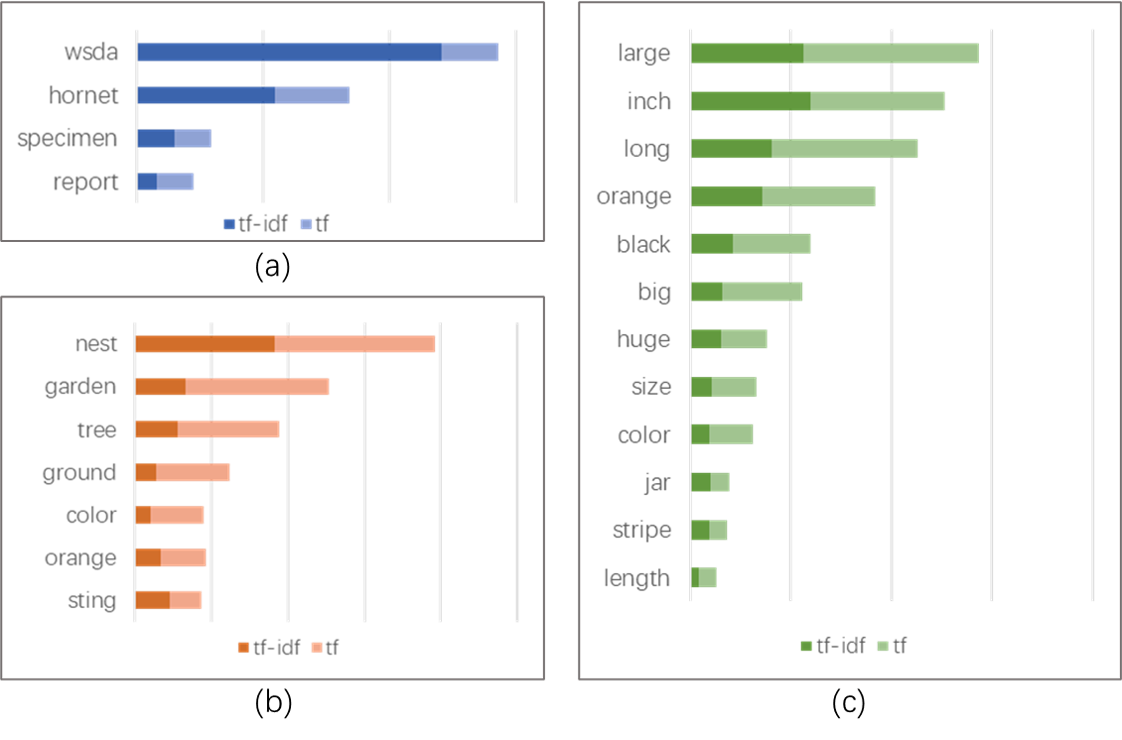
\includegraphics[width=12cm]{tfs.png}
    \caption{Terms of the highest TF-IDF scores.}
    \label{fig:tfs}
\end{figure}

Then, We subjectively selected the detailed description words from the top 100 most frequently used words in all report notes, \emph{e.g.} "large", "inch", "orange", "black", \emph{etc.}, which means the report is more likely to be along with detailed descriptions and thus more helpful for lab researchers to decide its status. Detailed results are shown in \autoref{fig:tfs} (b).

Next, when it comes to the lab comments of negative or unverified detection, they usually convey two kinds of information, including the actual species of the wasp detected and the reason for the negative judgment. Therefore, statistics are also conducted to lab comments of negative detection reports. After pattern matching with other species of high possibility to be mistaken (mentioned later), the rest of words turn out to be the features most likely to be misjudged for \VM, \emph{e.g.} "garden", "tree" are less likely to be the active area of \VM, while "orange" is the correction of the reported colors of "yellow" in notes (and thus we later replace "orange" with "yellow" in $MP$ corpus). Detailed results are shown in \autoref{fig:tfs} (c).


Based on the statistics above, we form the corpus of $CF$, $DT$, and $MP$, storing the most frequent terms under the three conditions mentioned above respectively.

\begin{table}[htbp]
    \centering
    \begin{subtable}{0.3\textwidth}
        \centering
        \begin{tabular}{cc}
            \toprule
            term & frequency \\
            \midrule
            WSDA & 0.0441 \\
            specimen & 0.0294 \\
            report & 0.0294 \\
            staff & 0.0147 \\
            \bottomrule
        \end{tabular}
        \caption{CF (High Confidence)}
        \label{subtab:cf}
    \end{subtable}
    \quad
    \begin{subtable}{0.3\textwidth}
        \centering
        \begin{tabular}{cc}
            \toprule
            term & frequency \\
            \midrule
            large & 0.0172 \\
            inch & 0.0133 \\
            orange & 0.0129 \\
            stripe & 0.0037 \\
            \bottomrule
        \end{tabular}
        \caption{DT (Detailed Description)}
        \label{subtab:dt}
    \end{subtable}
    \quad
    \begin{subtable}{0.3\textwidth}
        \centering
        \begin{tabular}{cc}
            \toprule
            term & frequency \\
            \midrule
            nest & 0.0168 \\
            garden & 0.0131 \\
            tree & 0.102 \\
            yellow & 0.0199 \\
            \bottomrule
        \end{tabular}
        \caption{MP (mistaken posibility)}
        \label{subtab:mp}
    \end{subtable}
    \caption{Excerpts from the corpus of different contexts.}
    \label{tab:test1}
\end{table}

Besides, we conduct pattern matching with common misjudged wasp species to lab comments for negative reports, from which to separate the real species of the wasp sighted. This provides ground truth labels for the following image classification task since the number of each class in the original data set is of severe imbalance. The numbers of each species are depicted in \autoref{fig:dataset-insect-pie}. 

\begin{figure}[htbp]
    \centering
    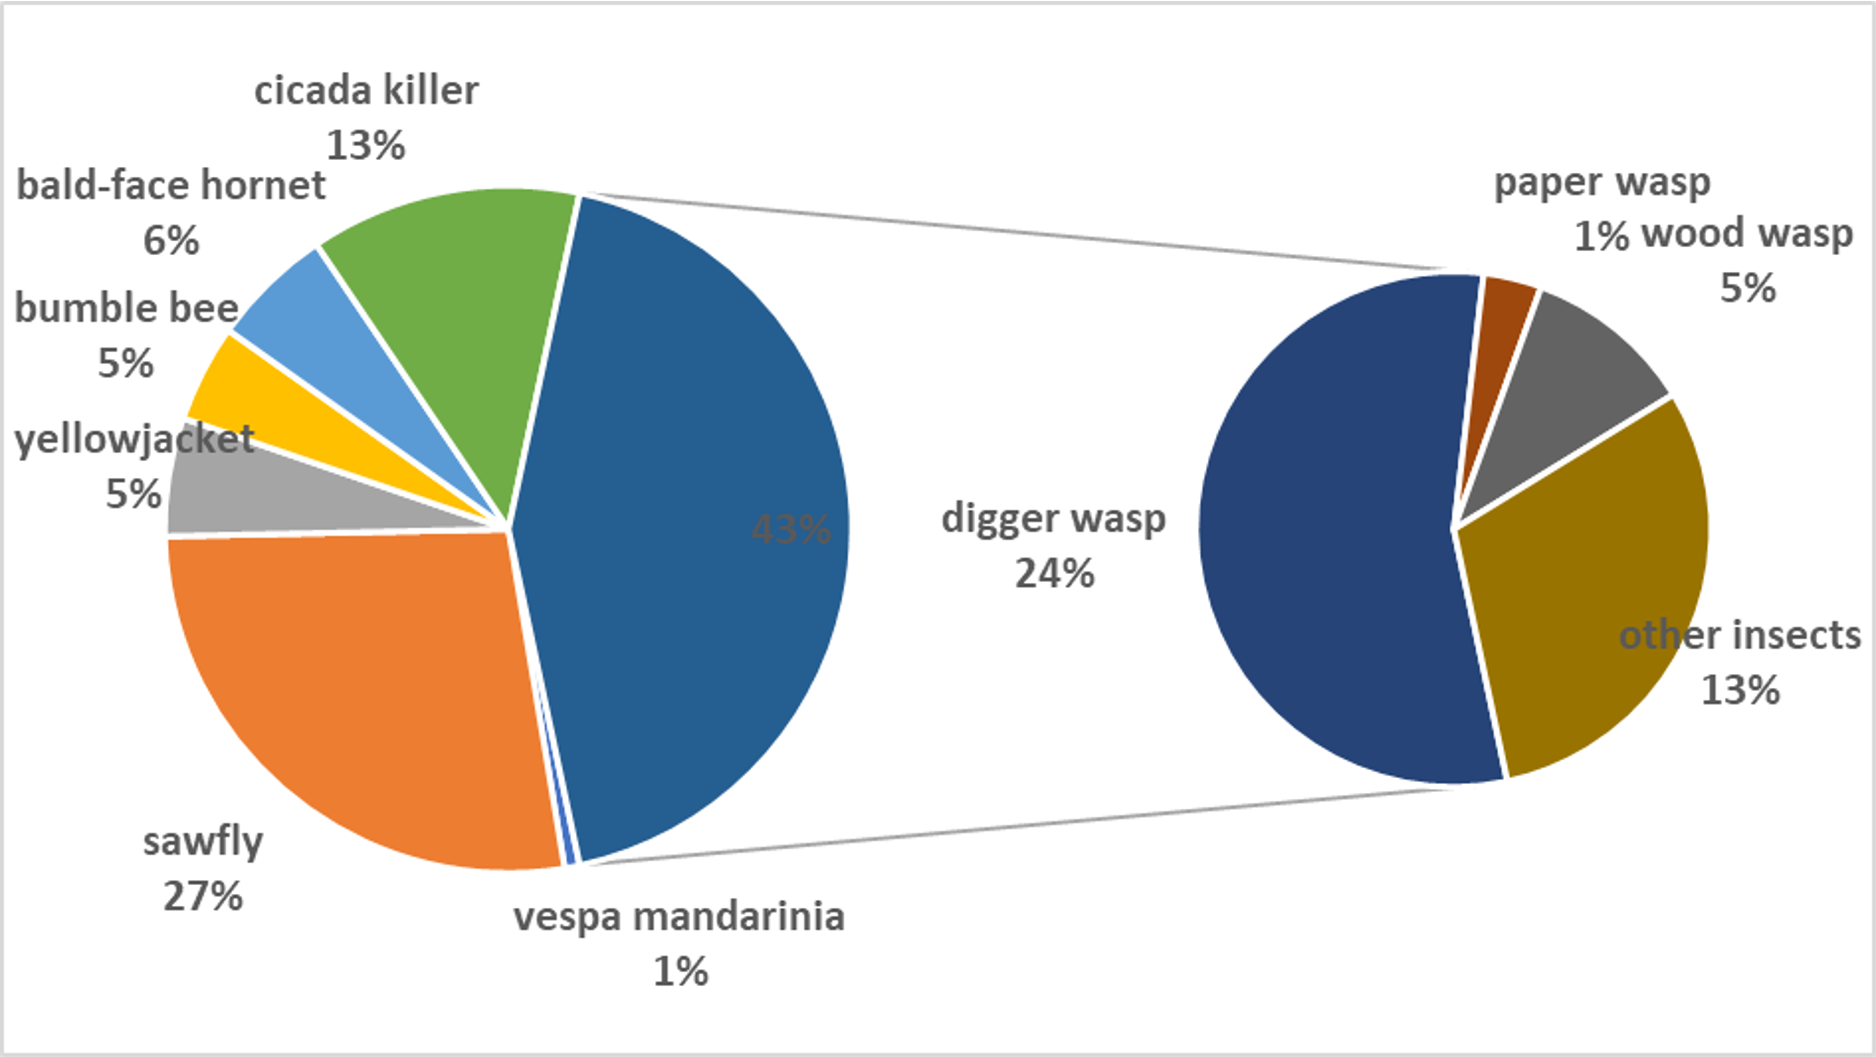
\includegraphics[width=12cm]{dataset-insect-pie.png}
    \caption{Percentage of insect type in all positive and negative reports.}
    \label{fig:dataset-insect-pie}
\end{figure}


\subsubsection{Bayes scoring strategy}

We apply the naive Bayes\cite{naivebayes} method to report notes based on the $CF$, $DT$, $MP$ corpus mentioned above. The Naive Bayes method is a conditional probability model, which  can be decomposed as:
\begin{eqnarray}
P(c \mid d) &=& \frac{P(d \mid c) \cdot P(c)}{P(d)} \nonumber\\
&\propto& P(d \mid c) \cdot P(c) \nonumber\\
&=& P(c) \ \prod_{k=0}^{n} P(t_k \mid c)
\end{eqnarray}
where $P(c \mid d)$ is the probability of document $d$ belonging to class $c$, and $P(c)$ is the prior probability of class $c$.

To simplify the model, we assign the weight of each class with $2$, $0.5$ and $-1$. Therefore, the textual scoring strategy can be expressed as:
\begin{eqnarray}
Score_{textual} = \sum_{k=0}^{n}weight_{t_k \in c} \cdot TF(t_k)
\end{eqnarray}
where $TF(t_k)$ is the term frequency of term $t_k$ in document $d$.


\subsection{Visual Recognition}
In 2013, AlexNet\cite{alexnet} used the CNN structure on the ImageNet\cite{imagenet_cvpr09} data set to defeat all traditional algorithms. Since then, CNN has become the mainstream method in image processing tasks. Compared with traditional algorithms that require feature engineering processing of pictures, CNN can learn the features of the classified objects by the neural network itself and iteratively update the network parameters.

We use Resnet18\cite{resnet} as our CNN backbone and introduce the idea of transfer learning\cite{transferlearning}. After loading the pre-trained weights of Resnet18 on ImageNet, we finetune the whole net on given data set and finally achieve a considerable effect.

Before we show the analysis results, there are several training details to be stated:
\subsubsection{Loss function}
During the training, we use Cross Entropy Loss (CE) as the loss function:
\begin{eqnarray}
loss(x,class)=- log(\frac{exp(x[class])}{\sum_j^{C-1}exp(x[j])}) = - x[class]+log( \sum_j^{C-1}exp(x[j]))
\end{eqnarray}

where C is the total number of categories.

\subsubsection{Normalization}
Because the images provided by the public are very different, such as different light intensity and color difference, we perform Gaussian normalization processing on all images, and the processed data obeys Gaussian distribution.
\begin{eqnarray}
x & = & \frac{x-\mu }{\sigma }
\end{eqnarray}
where $\mu$ and $\sigma$ are the mean and standard deviation of each picture.

\subsubsection{Training data}
We divide the data set, and the ratio is the N(training set): N(validation set)=6:4. The results of the division are shown in the \autoref{tab:dataset_proportion}. Our model is trained for 20 epoches(64 batches in each batch) with learning rate $\alpha$ =5e-4 and Adam optimizer.

\begin{table}[H]
    \centering
    \begin{tabular}{cccccc}
    %\begin{tabular}{|l|l|l|l|l|l|}
        \toprule
        Category   &bald face hornet  &bumble bee  &cicada killer  &digger wasp  &other insect \\ 
        \midrule
        %\hline
        Train      & 95               & 84         & 245           & 422         & 247         \\ 
        %\hline
        Validation & 63               & 55         & 162           & 280         & 163         \\ 
        %\hline
        Total      & 158              & 139        & 407           & 702         & 410         \\ 
        \bottomrule
        \vspace{0pt} \\
        \toprule
        Category   &paper wasp       &sawfly    &Vespa mandarinia  &wood wasp    &yellowjacket  \\ 
        \midrule
        %\hline
        Train      & 22              & 504      & 9                & 68          & 93           \\ 
        %\hline
        Validation & 13              & 335      & 5                & 45          & 61           \\ 
        %\hline
        Total      & 35              & 839      & 14               & 113         & 154          \\
        \bottomrule
    \end{tabular}
    \caption{The number of images in data set used in \VM\ recognition.}
    \label{tab:dataset_proportion}
\end{table}

Shown in \autoref{tab:CNNmodelacc}, our model achieves 63\% accuracy on the validation set and recognize 80\% of \VM, which demonstrates that our model has a strong ability of finding \VM. 
\begin{table}[H]
    \centering
    \begin{tabular}{cccccc} 
        \toprule
        Category &bald face hornet  &bumble bee  &cicada killer  &digger wasp  &other insect  \\ 
        \midrule
        Accuracy & 33.33\%          & 29.09\%    & 58.02\%       & 80.36\%     & 52.76\%      \\ 
        \bottomrule
        \vspace{0pt} \\
        \toprule
        Category &paper wasp        &sawfly    &Vespa mandarinia  &wood wasp   &yellowjacket  \\ 
        \midrule
        Accuracy & 30.77\%          & 80.00\%  & 80.00\%          & 8.89\%     & 39.34\%      \\
        \bottomrule
    \end{tabular}
    \caption{The accuracy of each category on validation set.}
    \label{tab:CNNmodelacc}
\end{table}

When it comes to the quantitative score, we use the convolutional neural network to run inference on each picture, and keep the value of the \VM\ category as the recognition score of the visual features of the picture.
\begin{eqnarray}
Score_{Recognition_i} & = & Value(Recognition\ Result_i(Vespa\ mandarinia))
\end{eqnarray}

\section{Problem 3: Score Ranking}
\subsection{Aggregation Method}
Based on the model of the second question, we score all the reported temporal-spatial data, textual data, and image data. We believe that the higher the temporal spatial correlation between a certain report and the positive reports, the more text keywords appear, and the more accurate image recognition, the more likely the report is positive sighting. Therefore, we sum the three scores and then sort all the scores to find the 25 reports with the highest score. It has to be mentioned that we normalize the three scores for the sake of fairness.

The formula for aggregation is as follows:
\begin{eqnarray}
Score & = & Score_{ST}+Score_{Textual}+Score_{Recognition}
\end{eqnarray}
Not surprisingly, all positive category scores are the highest, and 14 positive reports occupy the top 15 of the list. In addition to the positive category, there is also an unverified report ranked ninth, which shows that this report is very likely to be positive sighting. The top-25 highest score report is shown below in \autoref{fig:scorerank}:
\begin{figure}[h]
    \centering
    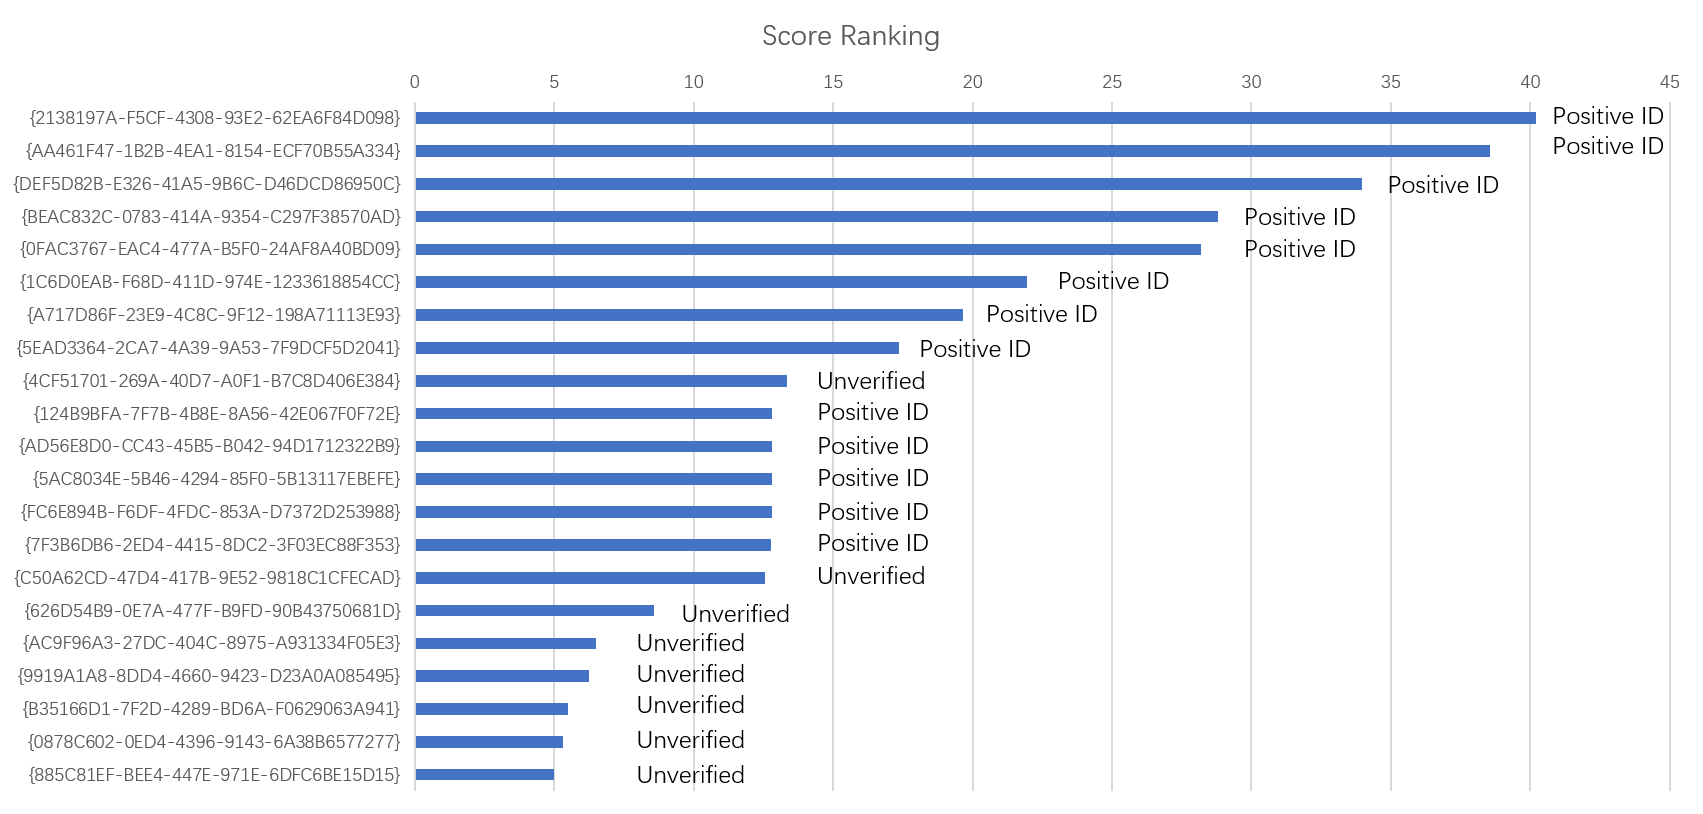
\includegraphics[width=\textwidth]{rank.png}
    \caption{Top 25 reports with highest scores.}
    \label{fig:scorerank}
\end{figure}

\subsection{Geographical Visualization}
Then we also visualize these points on a geographical map as shown in \autoref{fig:cluster}. The results show a high correlation and directly prove that our model works well.
\begin{figure}[h]
    \centering
    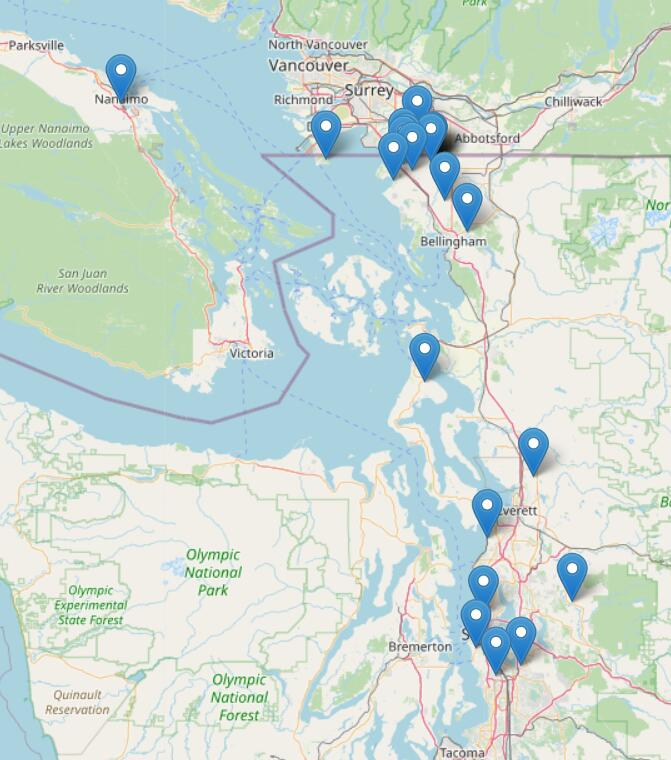
\includegraphics[width=8cm,height=6cm]{cluster.jpg}
    \caption{Visualization of 25 reports with the highest score on a geographical map.}
    \label{fig:cluster}
\end{figure}
We recommend that WSDA pay more attention to these 25 reports first, because they indicate that \VM\ may appear nearby.

\section{Problem 4: Model Entropy}
In this section, we will discuss the stability of START model. Obviously, it is an important question to update our model given additional new reports over time and decide how often the updates should occur.

We decided to discuss this matter in two aspects, and divide the report into two categories: high confidence and low confidence type. Specifically, the report clearly marked as positive or negative is defined as a report with high confidence; the report marked as unverified or unprocessed is defined as a report with low confidence.

\subsection{Data of High Confidence}
\label{section:highconfdata}
Since the data of the positive category is very scarce, we must make full use of it after we get a new report of positive, such as its images, location, and detection date, which will definitely help to track the trail of \VM. At the same time, negative reports can help CNN architecture better identify pictures of insects and indirectly strengthen the ability to find error reports. In addition, the densely appearing bee colonies in negative reports often represent the absence of \VM, because \VM\ will feed on other bee colonies. All in all, when the report is calibrated by researchers as positive or negative, we must retrain our network with the new data set. The specific method is as follows:
\begin{itemize}
    \item {Temporal spatial features:} Rerun the clustering algorithm and calculate the $ST_{score}$ of each point as discussed in Section  \ref{section:ST_analysis}.
    
    \item {Textual features:} Simply update the term frequency in $CF$, $DT$ and $MP$ corpus with the report notes, especially important for positive reports,
    
    \item {Recognition:} Divide the data set again using the new label of each image. The image attached to the negative report can be obtained in lab Comments column. Then load the existing model weight to continue training and set a small learning rate(\emph{e.g.} 5e-5) until the model converge again on the new data set.
\end{itemize}

\subsection{Data of Low Confidence}
Unverified and unprocessed data is very difficult to use for most models. An important reason is that it does not have a clear label, so we cannot predict its impact on the effect of the model. But START model has the ability of clustering points, so it can naturally identify information points and noise points. Based on this idea, we introduce the concept of model entropy to represent the stability of the model.

Entropy is often interpreted as the degree of disorder or randomness in the system. The term is used in diverse fields, from classical thermodynamics to the principles of information theory. We define the formula for model entropy as follows:
\begin{eqnarray}
Model\ Entropy & = & \frac{-\sum_{i =  0}^{N-1}  log(Score_{ST_i})}{N}
\end{eqnarray}
where N is the total number of points.

Then we manually make up some fake data in positive ID. An example is shown in the \autoref{tab:fakedata} below. The detection date is 1 day after the true report and the geographical distance is $ 0.01^\circ$ in both longitude and latitude, which ensures that the new report can be divided into the cluster.

\begin{table}[H]
    \centering
    \begin{tabular}{ccccc} 
        \toprule
        Status & Detection date & Lab status  & Longitude   & Latitude    \\ 
        \midrule
        True   & 2020-10-1      & positive ID & -122.582465 & 48.983375  \\ 
        %\hline
        Fake   & 2020-10-2      & positive ID & -122.592465 & 48.973375  \\
        \bottomrule
    \end{tabular}
    \caption{Manually make up fake data to check the stability of START model.}
    \label{tab:fakedata}
\end{table}

\begin{figure}[h]
    \centering
    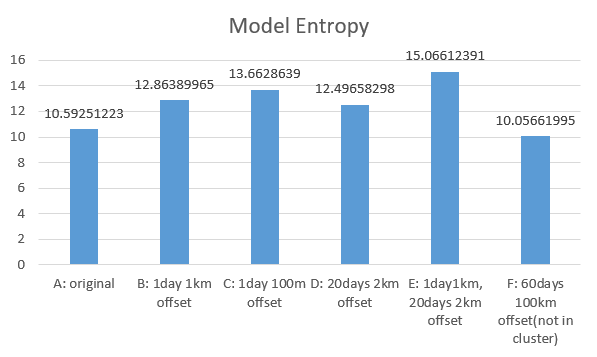
\includegraphics[]{entropy.png}
    \caption{Model entropy with different fake data.}
    \label{fig:entropy}
\end{figure}
We conduct five sets of controlled experiments, and the result is shown in \autoref{fig:entropy}. We find that the closer the newly inserted data is to the original data, the greater the entropy of the model (BCD); if two points are added to the cluster (E) at the same time, the model entropy will increase significantly. And if the newly added data is not related to the original data (F), then the model entropy will not increase, or even slightly decrease due to the increase of the number of points.

So, we safely conclude that once new reports come in, we can calculate the model entropy to measure the stability and accuracy of the START model. If the entropy increases sharply, we will regard the newly inserted point as positive data. Otherwise, it is a negative point. Based on empirical experience, when the new entropy is equal to 1.5 times the original entropy, we update the original model, and the updated plan refers to Section \ref{section:highconfdata}.

\section{Problem 5: Active Threshold}
In this section, we focus on the end of pest spread. We will discuss this issue in conjunction with the scoring mechanism of the START model and the life habits of the \VM.

According to the discussion of the third question, we will draw a line at the position of the score of the last positive report, and use this line as the active threshold of our system. Any report below this baseline score will be treated as negative. If a positive report appears in the updated data and the score is lower than the threshold, then we will re-update it to the lowest scoreline of the positive report scores. If there is no data that exceeds it for a long period of time, \emph{i.d.} two months, we believe that \VM\ has been completely extinct in Washington State. Two months is inaccurate, because we also need to consider \VM\  hibernation. 

According to the report \cite{AGH}, when Winter arrives, the current seasons' nests die out and only overwintering queens survive. Overwintering queens emerge in the spring and they find safe areas to begin building a nest. By August the hive is fully mature, with up to 100 worker bees. The queens produce drones in September. Drones and queens leave the nest to mate in October and early November.

So if the positive reports do not appear for two months in Winter, we cannot conclude that the pest has been eradicated in Washington State. We just skip the winter report. Starting from the next spring (roughly in March), if there is no report that exceeds the threshold of the system within two months, we can announce that the \VM\ is extinct. The pseudo-code is as follows.
\begin{breakablealgorithm}
  \caption{ Framework of constituting evidence that \VM\ is eradicated.}
  \label{alg:Framwork}
  \begin{algorithmic}[1]
    \Require
        The new reports including detection date, sighting location, notes, lab comments, lab status and images.
    \Ensure
        The conclusion whether \VM\ is eradicated or not.
    \State initial Counter=0, bottomline = $+\infty$
    \If{Counter == 0 in two month}
    \State return eradicated
    \EndIf
    \If{report submits in Winter}
    \State continue
    \Else
    \If{report.value < bottomline and report is not positive}
    \State continue
    \Else
    \State Counter += 1
    \If{report.value < bottomline}
    bottomline = report.value
    \EndIf
    \EndIf
    \EndIf
  \end{algorithmic}
\end{breakablealgorithm}

\section{Strengths and Weaknesses}
\subsection{Strengths}
\begin{itemize}
    \item \textbf{Strength 1}\\
    We use multi-modal technology to process data in different formats, including text, images, and geographic information.
    \begin{itemize}
    \item We use STDBScan to cluster temporal spatial data to find the degree of correlation between reports.
    \item We use lab comments to annotate image data categories and use LDA and TFIDF models to analyze the word frequency of notes to help us understand why people mistake other insects for \VM.
    \item We use CNN to train the annotated image data with 10 categories and achieve a good result on the validation set. The accurate recognition rate of \VM\ reaches 80\%.
    \end{itemize}
    \item \textbf{Strength 2}\\
    We use a scoring mechanism to integrate the above three scores, and the report with the highest score is considered the most likely positive sighting.
    \item \textbf{Strength 3}\\
    We introduce the concept of model entropy and regard the impact of new data on model entropy as an important factor in whether the model is worth updating.
    
\end{itemize}

\subsection{Weaknesses}
\begin{itemize}
    \item \textbf{weakness 1}\\
    Except for the first question, our model does not focus on biological characteristics in most cases, but only focuses on data features, such as temporal and spatial distribution, text description, and image appearance.
    \item \textbf{weakness 2}\\
    The problem of data imbalance limits the accuracy of our model.
    \item \textbf{weakness 3}\\
    Due to time constraints, in the text processing dictionary, our description dictionary of the \VM\ is not very complete.
\end{itemize}
\section{Conclusions}
From December 2019, the corpse of a \VM\ made people alert. With the arrival of a large number of reports carrying text, pictures, and geographic information, a new multi-modal solution needs to be proposed to find the most informative data from the complex data.

We use temporal spatial data clustering to track the trajectory of the \VM , and use the lab comments in the report to label the image data with category information. Then, we analyze the word frequencies of report notes to find out the mistaken classified reason. Further, a CNN network is used to process the annotated pictures. We fuse temporal spatial data, text feature, and visual feature scores to get the final report score. Based on this, we find the most valuable reports and submit our memorandum to WSDA.


\section{Memorandum}

\noindent \textbf{Date:}\ \ \today \\
\noindent \textbf{To:}\ \ Administrator, Washington State Department of Agriculture \\
\noindent \textbf{From:}\ \ Team \#\TeamNumber \\
\hrule \vspace{10pt}
\noindent
Chief Administrator,

    From December 2019, the discovery of \VM\ has made us all very alert and worried because it will harm local beneficial insects. Fortunately, the Washington State government announced a series of response measures in time, including allowing the public to submit reports of seeing \VM. But another problem has arisen. A large number of complex reports have stretched all WSDA staff, so we propose a model that can help you deal with multi-modal report data. Let me introduce the results of our research.
    \begin{itemize}
       \item \textbf{Consider sending more faculty to $\mathbf{48^\circ59'3''}$N, $\mathbf{57^\circ25'30''}$W.} \\
        We visualize the positive report result on a geographical map and find that the distances in space are less than $\pm 0.5^\circ$ in longitude(around 31 miles) and $\pm 0.2^\circ$ in latitude(around 12 miles). Then we use the STDBScan model to cluster the existing positive reports and get the most relevant reports in the temporal spatial data are concentrated in the $48^\circ59'3''N$ $57^\circ25'30''W$ area. Therefore, we recommend that WSDA send more personnel to the surrounding area to check if there are Vespa mandarinia gathering.

        \item \textbf{Score the report notes with our textual model.} \\
        Based on the analysis of report notes, we find out the words of strong correlation with high confidence, detailed description and mistaken possibility, and thus able to score the report notes according to their confidence and helpfulness. Our model then may serve as the filter for selecting the reports with high probability before processing by lab researchers and WSDA staffs, prioritizing the most informative and helpful ones.

        \item \textbf{Run our CNN model to identify \VM\ in thousands of images.} \\
        We mark the image data based on the existing text data and send the well-annotated data to the convolutional neural network, also named CNN. The number of this data set has reached about three thousand. CNN can achieve 63\% accuracy on the validation data set, and can accurately identify 80\% of \VM. With this good helper, I think the staff of WSDA will no longer have to worry about a large amount of image data.

        \item \textbf{Apply our aggregation score to get the most informative report quantitatively.} \\
        The multi-modal model we proposed can find the most informative report among all reports by scoring. Based on the scores of the above three aspects, we add them and then sort them, and we can easily get the most likely positive reports. With the guidance of this data, you can dispatch personnel to the most critical areas with the highest scores.
        
        \item \textbf{Use model entropy to process the unverified or unprocessed report.} \\
        Due to time limitations, the WSDA staff cannot handle all reports in time. Therefore, we propose the concept of model entropy to speed up the identification of unprocessed or unverified reports. We only need to observe whether a new report has a great impact on the model entropy. If it does, then it means that the report has great reference value. Otherwise, it means that the report has a low probability of being informative.
    \end{itemize}

We are really honored to provide you with a model for processing multi-modal data and finding the most informative reports. Hope our suggestions may help.

\noindent Sincerely yours, 

\noindent Team \#\TeamNumber

%============end thesis (main part)===============

\newpage
\bibliographystyle{unsrt} % reference按引用先后排序
\bibliography{refer} % build reference from file "refer.bib"


\begin{appendices}
\section{Selected Source Code}

\noindent \textbf{\tt \red{st\_dbscan.py}}
\lstinputlisting[language=Python]{./code/st_dbscan.py}

\noindent \textbf{\tt \red{GM(1,1) grey differential model predicting program}}
\lstinputlisting[language=Python]{./code/GM11.py}


\end{appendices}

\end{document}